% LaTeX Curriculum Vitae Template
%
% Copyright (C) 2004-2009 Jason Blevins <jrblevin@sdf.lonestar.org>
% http://jblevins.org/projects/cv-template/
%
% You may use use this document as a template to create your own CV
% and you may redistribute the source code freely. No attribution is
% required in any resulting documents. I do ask that you please leave
% this notice and the above URL in the source code if you choose to
% redistribute this file.

\documentclass[11pt,a4paper]{article}
\usepackage[utf8]{inputenc}
\usepackage[english]{babel}

\usepackage[left=2cm,right=2cm,top=1.5cm,bottom=1.5cm]{geometry}

\usepackage{hyperref}
\usepackage[usenames,dvipsnames]{color}
\usepackage{tabularx}
\usepackage{multirow}
\usepackage{graphicx}

% Comment the following lines to use the default Computer Modern font
% instead of the Palatino font provided by the mathpazo package.
% Remove the 'osf' bit if you don't like the old style figures.
\usepackage[T1]{fontenc}
\usepackage[sc,osf]{mathpazo}

\def\name{Onur Güzel}
\def\cv{Curriculum Vitae}

\author{\name}
\title{\cv}

\hypersetup{
  colorlinks = true,
  urlcolor = blue,
  pdfauthor = {\name},
  pdfkeywords = {programming, system administration, linux, open source},
  pdftitle = {\name: \cv},
  pdfsubject = {\cv},
  pdfpagemode = UseNone
}

% Custom section fonts
\usepackage{sectsty}
\sectionfont{\rmfamily\mdseries\Large\vspace{-10pt}}
\subsectionfont{\rmfamily\mdseries\itshape\large\vspace{-5pt}}

% Don't indent paragraphs.
\setlength\parindent{0em}

% Make lists without bullets
\renewenvironment{itemize}{
  \begin{list}{}{
    \setlength{\leftmargin}{0em}
  }
}{
  \end{list}
}

\begin{document}
\pagenumbering{gobble}

\begin{tabularx}{\textwidth}{ X r }
\multirow{6}{*}{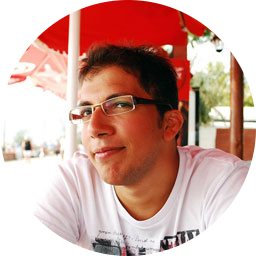
\includegraphics[scale=0.4]{photo}} & \\[0.5cm]
 & \Huge \name\\
 & \href{http://www.onurguzel.com/}{\tt onurguzel.com} - 
\href{mailto:guzelmu@gmail.com}{\tt guzelmu@gmail.com} - 
\href{http://onurguzel.com/twitter}{\tt @onurguzel}\\
 & \href{http://onurguzel.com/github}{\tt github} - 
\href{http://linkedin.com/in/guzelmu}{\tt linkedin} - 
\href{https://keybase.io/onurguzel}{\tt keybase} - 
\href{http://www.slideshare.net/onurguzel}{\tt slideshare} - 
\href{http://www.ohloh.net/accounts/onurguzel}{\tt ohloh}\\
 & GPG ID: AC5F 9E97 - tel: +90 536 414 4889\\
 & \\[0.5cm]
\end{tabularx}

\section*{About}
I'm an engineer who loves programming and open source software. I enjoy learning new skills about trending web and mobile technologies. I am enthusiastic about writing readable and reusable code to build scalable applications and automating \textit{everything}. Check out my profiles above.\\[10pt]
Born on November $4^{th}$, 1989 in Çanakkale, Turkey. Citizen of Republic of Turkey. Single.

\section*{Education}
\begin{itemize}
\item
\begin{tabularx}{\textwidth}{ l X r }
- & Master's degree, Business Administration & 2017 - present \\
& \textbf{Okan University} & \href{http://www.okan.edu.tr/en/}{okan.edu.tr}
\end{tabularx}
\item
\begin{tabularx}{\textwidth}{ l X r }
- & BS, Physics Engineering & 2007 - 2015 \\
& \textbf{Istanbul Technical University} & \href{http://www.itu.edu.tr/en/}{itu.edu.tr}
\end{tabularx}
\end{itemize}

\section*{Experience}
\subsection*{Employment}
\begin{itemize}
\item
\begin{tabularx}{\textwidth}{l X r}
- & Lead Software Engineer & February, 2015 - present\\
& \textbf{Artistanbul} & \href{https://www.artistanbul.io/}{artistanbul.io}
\end{tabularx}
\item
\begin{tabularx}{\textwidth}{l X r}
- & Web Development with Python \& Django Course Instructor & June, 2013 - present\\
& \textbf{yazılım24} & \href{http://yazilim24.com/}{yazilim24.com}
\end{tabularx}
\item
\begin{tabularx}{\textwidth}{l X r}
- & \textbf{Google} Summer of Code Student & April, 2013 - September, 2013\\
& \textbf{Fedora} Project & \href{http://fedoraproject.org/}{fedoraproject.org}
\end{tabularx}
\item
\begin{tabularx}{\textwidth}{l X r}
- & Part-time System Administrator & March, 2013 - May, 2013\\
& \textbf{National Center for High Performance Computing} & \href{http://www.uhem.itu.edu.tr/}{uhem.itu.edu.tr}
\end{tabularx}
\item
\begin{tabularx}{\textwidth}{l X r}
- & Contributor at \textbf{Pardus} GNU/Linux Project & March, 2010 - January, 2012\\
& Center of Research for Advanced Technologies of Informatics and Security (\textbf{BİLGEM}), The Scientific and Technological Research Council of Turkey (\textbf{TÜBİTAK}) & \href{http://bilgem.tubitak.gov.tr}{bilgem.tubitak.gov.tr}
\end{tabularx}
\item
\begin{tabularx}{\textwidth}{l X r}
- & Co-founder, Software developer and System Administrator & September, 2009 - present\\
& \textbf{arı24} (formerly İTÜ24) - Newspaper of Istanbul Technical Univ. & \href{http://ari24.com}{ari24.com}
\end{tabularx}
\end{itemize}

\subsection*{Skills}
\begin{tabularx}{\textwidth}{l l X}
- & Languages: & Python, JavaScript, PHP, Java\\
- & Databases: & PostgreSQL, MySQL, MongoDB, Redis, Memcache\\
- & Frameworks and SDKs: & Django, Django REST Framework, React, Android SDK, CakePHP\\
- & Other: & docker, git, vim, webpack, nginx, php-fpm, gunicorn, supervisord
\end{tabularx}

\subsection*{Honors \& Awards}
\begin{tabularx}{\textwidth}{l X r}
- & Certificate of Appreciation & 2010\\
& UEKAE, TÜBİTAK
\end{tabularx}

\vspace{10pt}
\footnotesize {\color[gray]{0.25} Last updated: December $12^{th}$, 2016. Latest version of this document can always be found at \href{http://onurguzel.com/cv}{\color{black}onurguzel.com/cv}}
\end{document}
